\section{Discussion}

Benchmarks serve as our proxies for AI capabilities in the wild; contamination breaks this proxy, creating an illusion of competence.
This work provides the first targeted examination of contamination in generative tasks.
While generative contamination shares the superficial signature of inflating scores, the underlying mechanism is distinct: it relies on fragile, verbatim memorization of long token chains that behaves fundamentally differently from robust reasoning.

Our scaling laws reveals the magnitude of this threat. Under standard scaling law assumptions, a single replica of the test set allows a model to bypass the estimated ``irreducible error'' barrier, achieving performance that would otherwise require more than an infinite amount of compute on uncontaminated data. However, this performance is brittle; critical ``levers'' -- sampling temperature and solution length -- differentiate memorization from generalization.
% Unlike robust reasoning, which survives stochastic sampling, contamination-driven performance collapses under high temperatures. Similarly, the shift from power law to exponential decay in performance as solution length increases signals the limits of the model's ability to hold a memorized chain without decoherence.

\begin{figure}[t!]
    \centering
    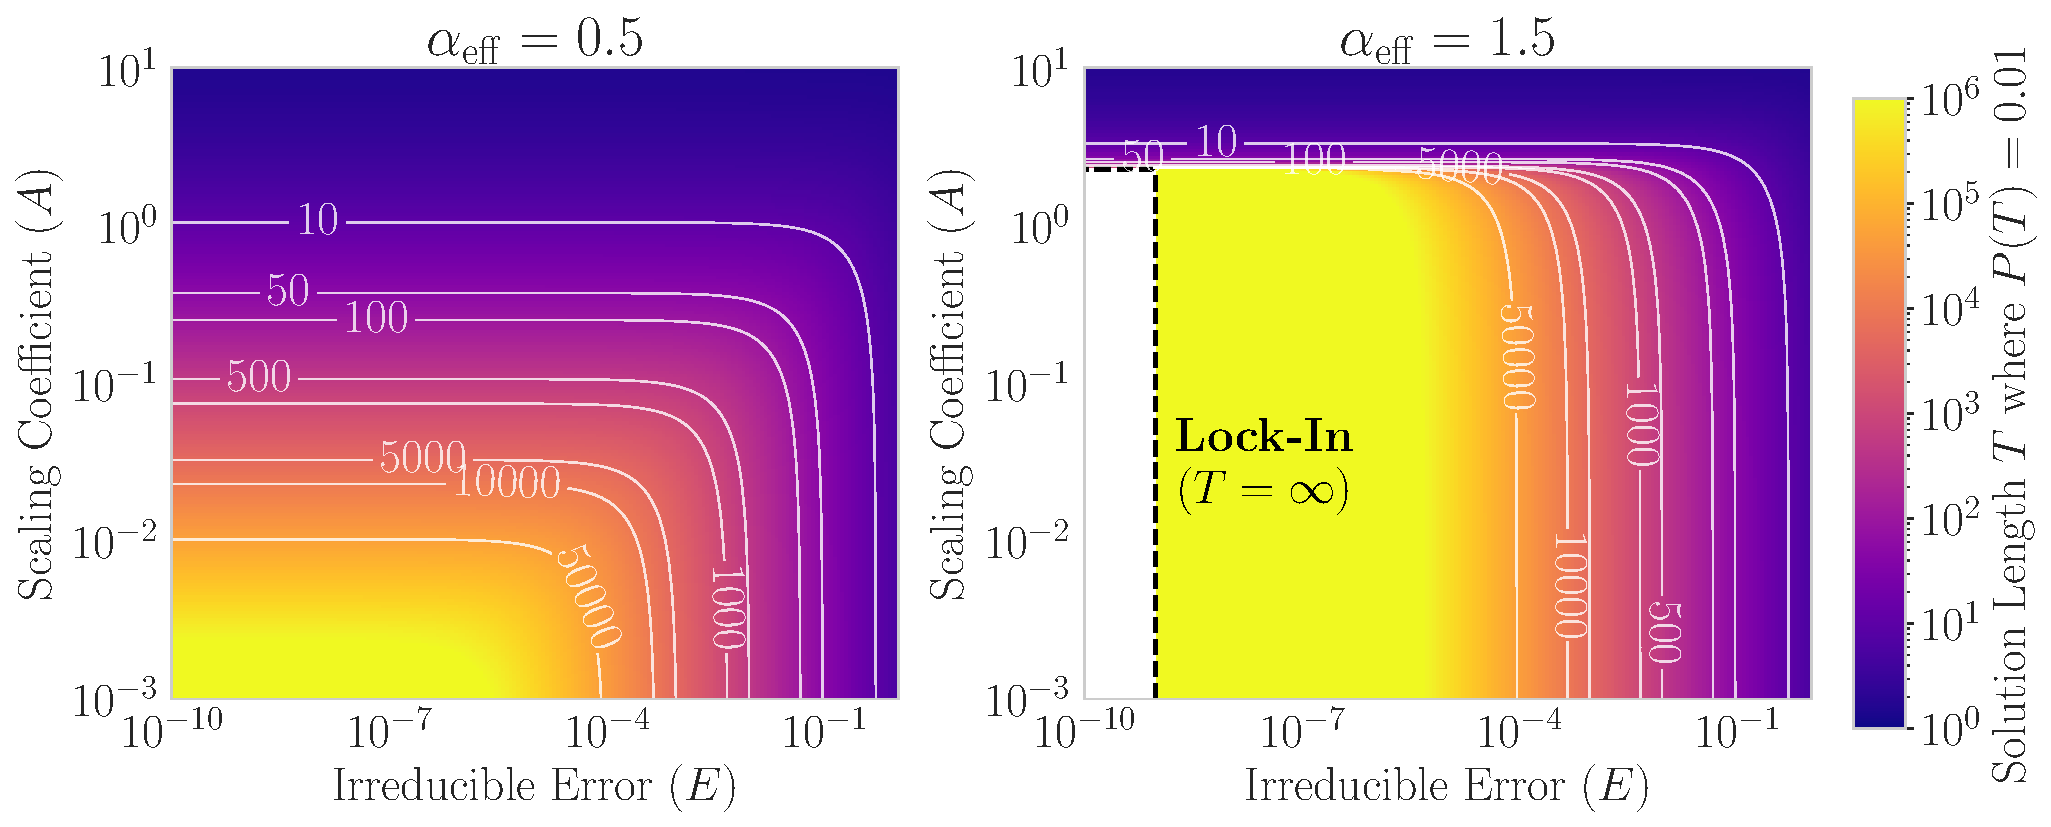
\includegraphics[width=0.9\columnwidth]{figures/50/phase_diagram_y=A_x=E_hue=T_alpha=multi_p=0.01.pdf}
    \caption{\textbf{Regimes of Memorization.} 
    Phase diagrams illustrating the maximum sustainable solution length $T$ for a fixed survival probability $P(T) = 0.01$. The three regimes are (1) Exponentially Fast Decoherence, (2) Brittle Memorization, and (3) Deterministic Lock-In.}
    \label{fig:phase_diagram}
\end{figure}

Perhaps most critically for practitioners, training pipelines can mask or expose this issue in counter-intuitive ways. The interaction between contamination and further training is governed by a ``dose-response'' effect \citep{schaeffer2025doseresponse, wei2025hubblemodelsuiteadvance}: overtraining on fresh data dilutes the contamination, and SFT on training data can degrade test performance by overwriting memorized test problems.
This implies that a drop in test accuracy after SFT, usually a sign of alignment tax or forgetting, may actually be a positive signal of decontamination.


\paragraph{Limitations.}
Our study isolates contamination on MATH, a single automatically verifiable generative benchmark, using decoder-only dense Qwen 3 models up to 344M parameters and one web-crawl pretraining mixture.
These choices make the causal study controlled, but they limit direct extrapolation to larger frontier models, other architectures, and other generative domains; Appendix~\ref{app:sec:discussion} discusses additional limitations and future directions.
